\chapter{Image Generation with GANs}\label{ch:generation}

    In this chapter we elaborate on the different methods that were employed to produce images from the extracted features. An arbitrary dataset of images can be used here, we went with \citetitle{102flower}~\cite{102flower}, a dataset of 102 different types of flowers containing slightly over 8000 images with a resolution of at least 512 x 512.\\
    Initially, we trained the generators on latent vectors generated from a multivariate normal distribution with 128, 16, or 32 dimensions for raw melspectrograms, autoencoder, and CRNN respectively. While this lead to good samples during training, generating images with latent vectors drawn from actual songs should generally not produce proper imges. The reason for this is that a multivariate normal distribution is very different to the distribution of latent vectors in songs. Since we needed to represent the distribution properly during training, a pretrained autoencoder or CRNN was used during the training of the generators. Figure~\ref{fig:distribution} displays an images generated from a generator that was trained on the proper distribution. While the first image was generated with a sample from a song, the second image was generated by drawing a latent vector from a multivariate normal distribution. These samples were generated after 125 epochs of training.

    \begin{figure}[h]
        \centering
        \subcaptionbox{\label{sfig:fixed_125}}{
            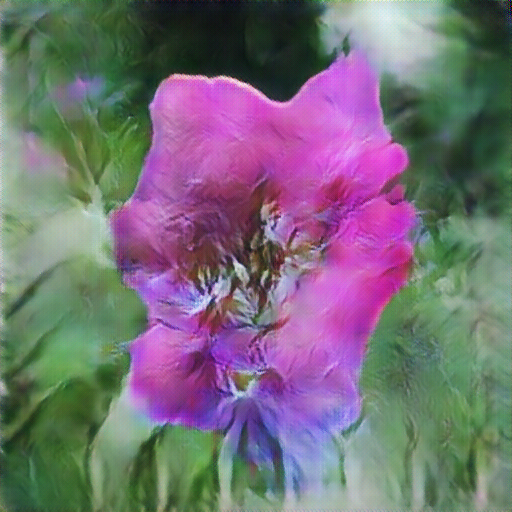
\includegraphics[width=.47\textwidth]{images/fixed_125_1}
        }
        \subcaptionbox{\label{sfig:rnd_125}}{
            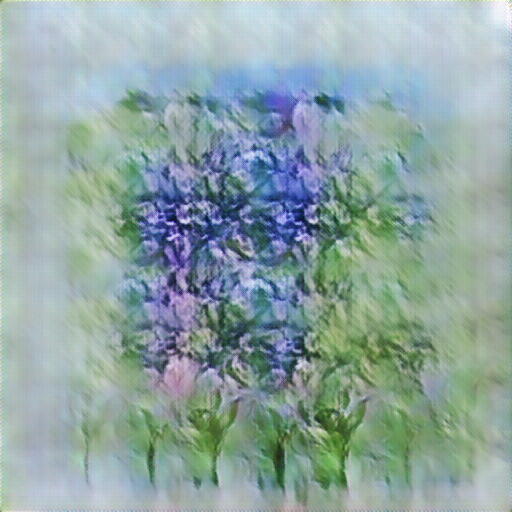
\includegraphics[width=.47\textwidth]{images/randomstatic_125}
        }
        \caption[Image generation with latent vectors from different distributions]
        {
            \textbf{Image generation with latent vectors from different distributions. The generator was trained on the distribution from the FMA dataset~\cite{FMA}. A latent vector from the proper distribution~\subref{sfig:fixed_125} and from a multivariate normal distribution~\subref{sfig:rnd_125}.}
        }
        \label{fig:distribution}
    \end{figure}
    
    \section{DCGAN}

        Instead of pooling layers DCGAN uses convolutional layers in the discriminator to reduce the image resolution and transposed convolutional layers in the generator to increase the image resolution, an example can be seen in Figure~\ref{fig:architecture_dcgan}.
        
        \begin{figure}[h]
            \centering
            \fbox{
                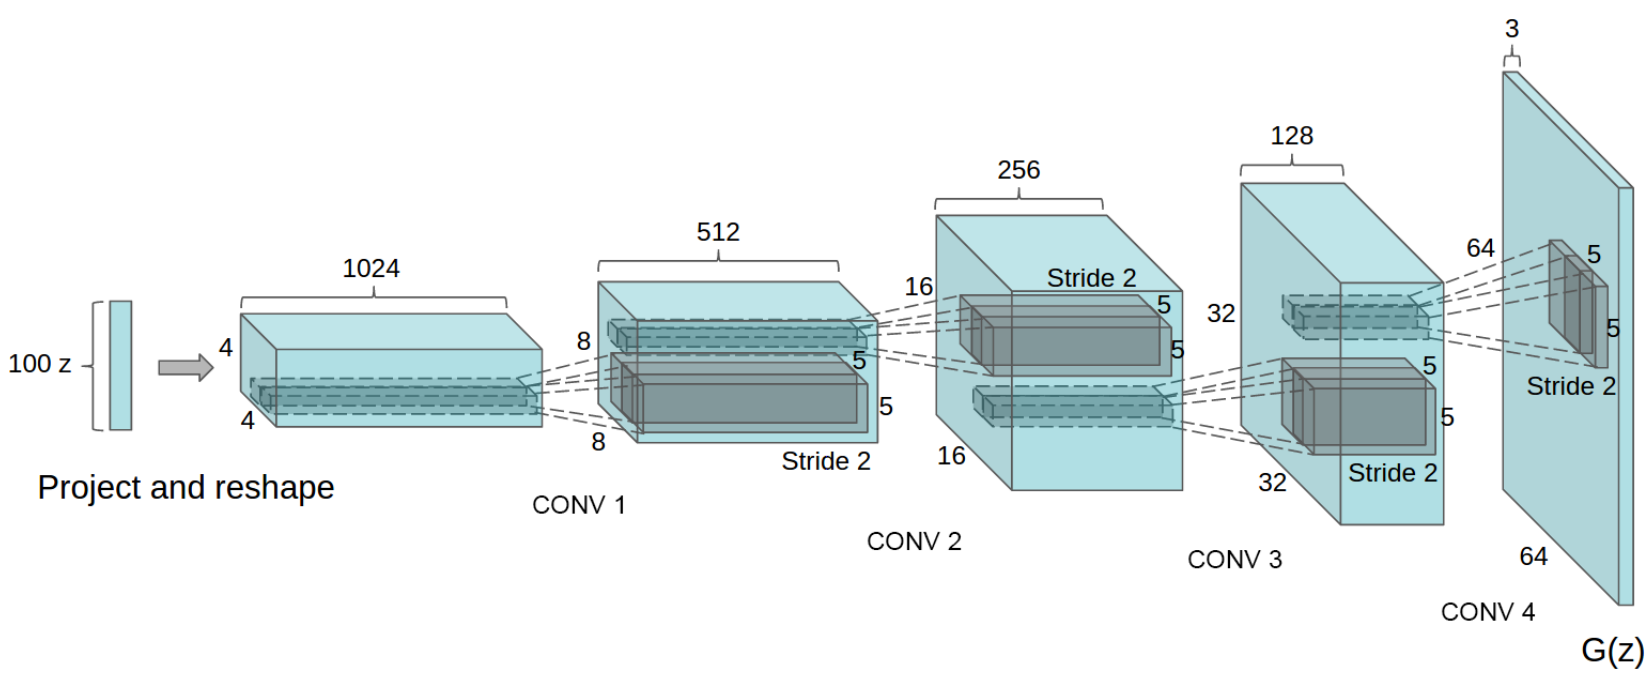
\includegraphics[width=.94\textwidth]{images/architecture_dcgan}
            }
            \caption[DCGAN generator for LSUN]
            {
                \textbf{DCGAN generator used for LSUN scene modeling. A 100 dimensional uniform distribution \vec{Z} is projected to a small spatial extent convolutional representation with many feature maps. A series of four fractionally-strided convolutions (in some recent papers, these are wrongly called deconvolutions) then convert this high level representation into a 64 × 64 pixel image. Notably, no fully connected or pooling layers are used.\\
                \textit{Figure and caption from} \citetitle{dcgan}~\cite{dcgan}.}
            }
            \label{fig:architecture_dcgan}
        \end{figure}

        Our first implementation was based on an implementation for CIFAR10. Because we want images with a resolution of more than 32 x 32, we scaled up the networks to fit our requirements.

        \subsection{Generator}

            As the input resolution for the generator is essentially 1 x 1, the first transposed convolutional layer of the generator, with a kernel size of 4, a stride of 1, and a padding of 0, outputs a resolution of 4 x 4. With an exception of the last, the remaining transposed convolutional layers double the resolution by instead using a stride of 2 and padding of 1 with the same kernel size. The last one uses a kernel size and stride of 1 and padding of 0, it is simply used ot reduce the channels for the final image, in our case 3.
            
            To reach our desired resolution of 512 x 512, we opted to increase the amount of layers rather than modify the stride and kernel size. This lead to an increase of transposed convolutional layers from 5 to 9. With the first and last having their own role, this leads to 7 layers doubling the resolution of 4 x 4 ($\rightarrow 4 \times 2^7 = 512$). While the original version reduced the amount of channels by a factor of two after each transposed convolutional layer, due to hardware limitations this method was no longer feasible after increasing the amount of layers. Instead we therefore reduced the amount of channels in the generator linearly. Due to a mistake during the first implementation and to keep backwards compatability, the last layer in the generator is scaled with 2$\times$ngf instead of 2$\times$ngf, with ngf being a variable that controls the size of the network. Each layers amount of output channels decreases in a linear fashion, with layer 8 having 2$\times$ngf filters, layer 7 has 4$\times$ngf, layer 6 has 6$\times$ngf, .., and layer 1 has 16$\times$ngf. The final architecture of our generator is displayed in figure~\ref{fig:architecture_dcgan_ours_generator}
        
            \begin{figure}[h]
                \centering
                \fbox{
                    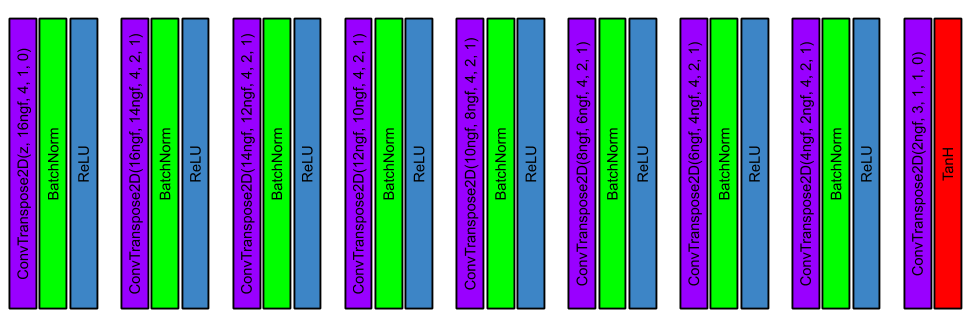
\includegraphics[width=.94\textwidth]{images/architecture_dcgan_ours_generator}
                }
                \caption[DCGAN generator architecture]
                {
                    \textbf{Architecture of our DCGAN generator that can be scaled with ngf and has a variable size of the latent vector \vec{z}.}
                }
                \label{fig:architecture_dcgan_ours_generator}
            \end{figure}

        \subsection{Discriminator}

            For the discriminator we applied the same approach. While the generator network increases the resolution while decreasing the amount of channels, the discriminator reduces the resolution and increases the amount of channels. The first convolutional layer starts out with the 3 input channels of an image, which are then increased linearly as we progress through the network. The exact architecture can be seen in figure~\ref{fig:architecture_dcgan_ours_discriminator}. Since the smallest transposed convolutional layer in the generator has 2$\times$ngf filters while the discriminators smallest convolutional layer has $\times$ndf filters, the generators network is more complex by default when ngf=ndf.

            \begin{figure}[h]
                \centering
                \fbox{
                    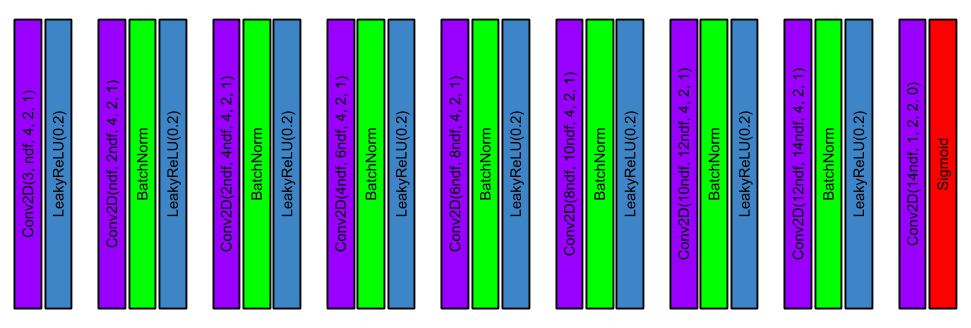
\includegraphics[width=.94\textwidth]{images/architecture_dcgan_ours_discriminator}
                }
                \caption[DCGAN discriminator architecture]
                {
                    \textbf{Architecture of our DCGAN discriminator that can be scaled with ndf.}
                }
                \label{fig:architecture_dcgan_ours_discriminator}
            \end{figure}

        \subsection{Training}
            As usual in adversarial nets, the generator and discriminator are competing against each other. We used Binary Cross Entropy Loss and the Adam optimizer for both networks. The discriminator is trained to distinguish between real images from the dataset and the images generated by the generator. The generator is trained through the discriminator, with the generators loss decreasing when the discriminator becomes worse at distinguishing the generated images from the real ones. The training of both networks can be summed up by the following minimax game where the generator tries to minimze and the discriminator tries to maximize the function~\cite{gan}

            \begin{equation}
                \min_D \max_G f(D, G) =
                \mathbb{E}_{\vec{x} \sim p_{\text{data}}}
                    \bigl[ \log D(\vec{x}) \bigr] +
                \mathbb{E}_{\vec{z} \sim p_z}
                    \bigl[ \log \left( 1 - D(G(\vec{x})) \right) \bigr].
                \label{eq:gan_1}
            \end{equation}

            Here, $\log D(\vec{x})$ is the log-likelihood of $\vec{x}$ being a sample from the dataset rather than a generated sample produced by the generator. When the discriminator reaches its optimum, or in other words, when it can perfectly distinguish the generated samples from the real samples, equation~\ref{eq:gan_1} can be reformulated to focus on the generator:

            \begin{equation}
                \mathbb{E}_{\vec{x} \sim p_{\text{data}}}
                    \bigl[ \log D(\vec{x}) \bigr] +
                \mathbb{E}_{\vec{x} \sim p_{\text{generator}}}
                    \bigl[ \log \left( 1 - D(\vec{x}) \right) \bigr]
                \label{eq:gan_2}
            \end{equation}

            Equation~\ref{eq:gan_2} reaches its maximum when $p_{generator}$ approaches $p_{data}$. As $p_{generator}$ is dependant on the latent vector $\vec{z}$, we can see that exchanging the distribution $p_{\vec{z}}$ after training will also change $p_{generator}$. As mentioned at the beginning of this chapter we therefore have to train with the correct distribution in latent space. In our case this means that we sample from the songs of the FMA dataset~\cite{FMA}, directly or after preprocessing them as described in chapter~\ref{ch:extraction}.

            As our music dataset contains roughly 8000 sample songs, with about 1800 possible valid latent vectors per song, we are drawing from a pool of $\num{1.44e7}$ samples. As each epoch is composed of our roughly 8000 images, we only draw as many latent vector samples. This means we only cover about $0.0556\%$ of our valid latent vectors. Additionally we draw exactly one sample from each song per epoch. This implementation may have an impact on our ability to model $p_{\vec{z}}$ correctly.

            Because of our implementation, using the same value for ngf and ndf, already leads to a generator that is about twice the size of the discriminator. During training we assumed that suitable values for ngf are 2$\times$ndf, with ndf at 32 and 64 leading to generated images of sufficient quality. At the time of writing, we realize that the discriminator should not necessarily be less complex than the generator. We are training some new networks with differently sized discriminators to help us understand the relationship between the complexity of the two networks. As training progressed we lowered the learning rates for both networks. We also ended up changing the value for the label of real images from 1.0 to 0.9. As the discriminators last layer is a sigmoid layer, the possible output ranges from 0 to 1. With this change the discriminator is discouraged to be overconfident. This should prevent the discriminator from making a decision based on a small set of criteria.

            When it came to producing videos based on songs, we realized that the samples of generated during training are not necessarily a good representation for how the final result will turn out. As we used randomly selected samples from $p_{\vec{z}}$, a trained generator might seem very promising while the frequent and important configurations for $\vec{z}$ produce disappointing results. The reason for this might be our bad modeling of $p_{\vec{z}}$. To allow us to better approximate the quality of the resulting videos, we modified our sample generation during training to produce some images from static latent vectors, which we know are relevant. For example, one of those is the latent vector representing the absence of sound. This static vector of course has to be different depending on the preprocessing of the melspectrograms.

            We struggled a lot with mode collapse during training. Attempting to reduce the learning rate in response yielded moderate improvements. It should be noted, that this problem was very persistent when using the encoded features, leading us to think that the 16-dimensional input vector just doesn't contain enough information. An example of mode collapse is shown in figure~\ref{fig:mode_collapse}

            \begin{figure}[h]
                \centering
                \includegraphics[width=.94\textwidth]{images/mode_collapse}
                \caption[DCGAN mode collapse]
                {
                    \textbf{Mode collapse when training a DCGAN}
                }
                \label{fig:mode_collapse}
            \end{figure}

    \section{InfoGAN}
        
        As we could not produce satisfying results with an InfoGAN we will not go too deep into its inner workings. The basic idea is to split the generators input into two parts, the latent vector and now additionally the latent code. The first part behaves the same as in a DCGAN, the latent code is supposed to represent specific features of the generated images. In the case of our flower dataset one parameter could for example be corresponding to the size of the generated flower. As explained in \citetitle{infogan}~\cite{infogan}, mutual information between the latent code and the generated images is maximized. This can be approximated by letting the descriminator attempt to extract the latent code that was used to create an image. The paper distinguishes between categorical and continuous latent code, e.g. in the case of MNIST the 10 different numbers can be mapped to categorical code with 10 classes. For our flowers we have opted to only use continuous code as our available inputs for the gennerator are all continuous variables.

        All our attempts at training an InfoGan were performed with the encoded 16 features produced from our autoencoder, the latent vector had a dimensionality of 84, summing it up to 100. In the first iteration we used Upsample layers to increase the image resolution while progressing through the generator. Even after increasing the amount of layers and / or the complexity of the networks, the results were extremely unsatisfying, even after tweaking the parameters and training multiple models. The second approach was to replace those layers with transposed convolutional layers and essentially use the DCGAN, which has proven to produce acceptable results, as a base for the new InfoGAN architecture. A comparison of both iterations can be seen in figure~\ref{fig:infogan_res_1}. All versions were implemented with MSELoss and the Adam optimizer.

        \begin{figure}[h]
            \centering
            \subcaptionbox{\label{sfig:infogan_trash}}{
                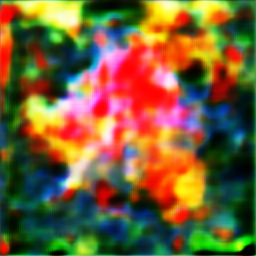
\includegraphics[width=.47\textwidth]{images/infogan_trash}
            }
            \subcaptionbox{\label{sfig:infogan_ok}}{
                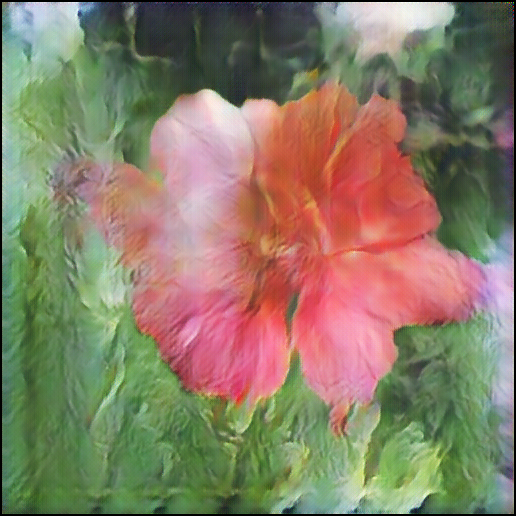
\includegraphics[width=.47\textwidth]{images/infogan_ok}
            }
            \caption[Images generated from InfoGans with different architectures.]
            {
                \textbf{Images generated from InfoGans with different architectures. \subref{sfig:infogan_trash} displays an image generated from the first iteration using Upsammple layers. \subref{sfig:infogan_ok} shows the second iteration that uses a very similar architecture to the DCGAN.}
            }
            \label{fig:infogan_res_1}
        \end{figure}

        While the second iteration of our InfoGAN implementation produced images of sufficient quality, another issue arose. As the idea is to have each dimension of the latent code correlate to an important property of the resulting image, our hopes were for the beat to correlate to for example the color or the size of the generated image. In figure~\ref{fig:infogan_res_2} 4 images can be seen that were generated with static latent code which was retrieved specific timesteps in a song that should produce 4 distinctly different images. It is clearly visible, that there are only very minor changes, e.g. the extend of the flower to the right. We have not investigated this any further as of now, so we can only speculate about the reasons for this behaviour. This could be a mode collapse, although more sample generation is necessary. Another reason could be that our implementation of the mutual information loss is faulty, leading to the generator simply ignoring the latent code. Finding out what, if anything, the model has encoded in the latent code requires more analysis.
        
        \begin{figure}[h]
            \centering
            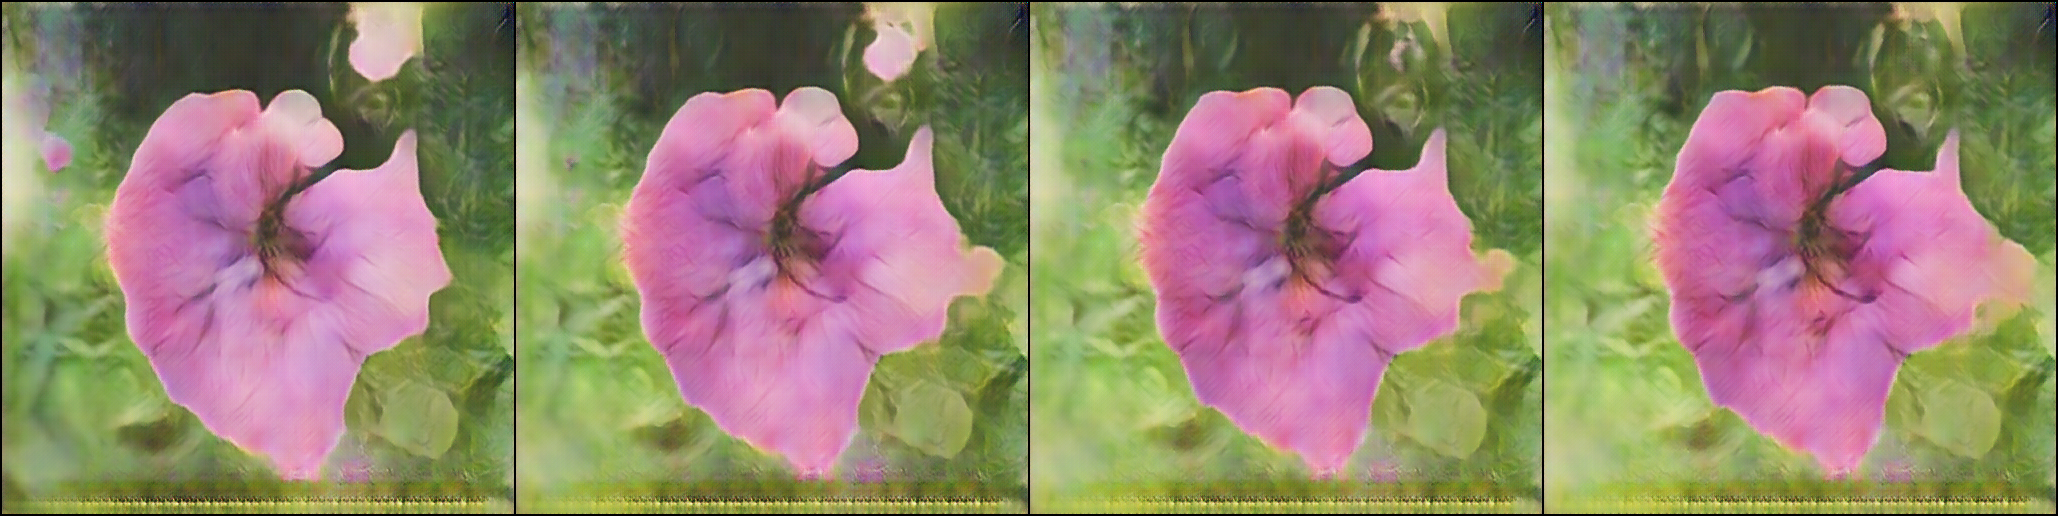
\includegraphics[width=.94\textwidth]{images/fixed_160}
            \caption[Images generated from InfoGan.]
            {
                \textbf{Visible are 4 images that were generated with an InfoGAN. The latent code used to produce these images was extracted from specific timesteps in a song that should produce visibly different images.}
            }
            \label{fig:infogan_res_2}
        \end{figure}